\documentclass[11pt]{article}
\usepackage{amsmath,amssymb,amsthm}
\usepackage{mathtools}
\usepackage{tikz}
\usepackage{enumitem}
\usepackage[margin=1in]{geometry}

\newtheorem{theorem}{Theorem}
\newtheorem*{theorem*}{Theorem}
\newtheorem{lemma}{Lemma}
\newtheorem{definition}{Definition}
\newtheorem*{definition*}{Definition}
\newtheorem{proposition}{Proposition}
\newtheorem{remark}{Remark}



\title{Math 106 -- Notes \\ Week 1: January 9, 2026}
\author{Ethan Levien}
\date{}

\begin{document}
\maketitle

\section*{Review}
On Thursday's class we reviewed some basic probability theory (probability spaces, probability measures etc.) and I introduced Markov chains. We saw the Chapman-Kolmogorov equation. You should try to prove it yourself. 

\section*{Invariant Distributions}

Let $P$ be a stochastic matrix on a finite state space $\Omega = \{1,\dots,I\}$ (in the book they use $S$).

\begin{definition*}
A probability vector $\pi$ is an \emph{invariant distribution} if
\begin{equation}
\pi = \pi P.
\end{equation}
\end{definition*}

Two basic questions:
\begin{enumerate}[label=(\roman*)]
\item When does an invariant distribution exist? (We know that $1$ is an eigenvalue since $P{\bf 1} = {\bf 1}$, thus the question is about whether the left eigenvector for this eigenvalue has positive entries and thus can be normalized). 
\item When is it unique?
\end{enumerate}
In Thursday's class I proved L3.5, which says the spectral radius is 1 for a stochastic matrix. 

\section*{Permutation Matrices and Relabeling}

\begin{definition*}[Not in book]
A \emph{permutation matrix} $R\in\mathbb{R}^{I\times I}$ has exactly one entry equal to $1$ in each row and column, and zeros elsewhere. In other words, $R_{i,j} \in \{0,1\}$ and $\sum_{i \in \Omega}R_{i,j}  = \sum_{j \in \Omega}R_{i,j} = 1$. 
\end{definition*}

Such a matrix corresponds to a permutation, that is, a bijection $\sigma:\Omega \to \Omega$ via 
\begin{equation}
R= \begin{bmatrix}
{\bf e}_{\sigma(1)} & \cdots & {\bf e}_{\sigma(I)}
\end{bmatrix}
\end{equation}
Note that $R{\bf e}_i = {\bf e}_{\sigma(i)}$ and $R^T{\bf e}_{\sigma(i)} = {\bf e}_i$. 
Thus, Permutation matrices are orthogonal: $R^{-1}=R^T$.  Note that $R^T$ is a permutation matrix as well. 
A permutation matrix corresponds to a relabeling of the states
\begin{equation}
\tilde{P} = R^T P R = R^{-1}PR. 
\end{equation}
Here, $R$ permutes the states, then $P$ is applied, then $R^T$ returns it to the permuted states. 


\section*{Reducibility and Irreducibility}

\begin{definition*}[D3.6]
A Markov chain with transition matrix $P$ is \emph{reducible} if there exists a permutation matrix $R$ such that
\begin{equation}
R P R^T =
\begin{pmatrix}
A_1 & B \\
0 & A_2
\end{pmatrix},
\end{equation}
where $A_1,A_2$ are square stochastic matrices of the appropriate dimensions. Otherwise, the chain is \emph{irreducible}.
\end{definition*}
We can think of the block decomposition as corresponding to a decomposition of the state space $\Omega = \Omega_1 \cup \Omega_2 = \{1,\dots,I_1\} \cup \{I_1 + 1,\dots,I\}$. Then, for example, $A_1$ would be a $I_1\times I_1$ matrix representing Markov transitions in $A_1$. 

\subsection*{Graph interpretation}

A Markov chain is irreducible if and only if, in the directed graph with edges
$i\to j$ whenever $P_{ij}>0$, there exists a path from any state to any other state.

\section*{Example}

Consider
\begin{equation}
P =
\begin{pmatrix}
\tfrac12 & \tfrac12 & 0\\
\tfrac14 & \tfrac12 & \tfrac14\\
\tfrac12 & 0 & \tfrac12
\end{pmatrix}.
\end{equation}

The associated transition graph is:

\begin{center}
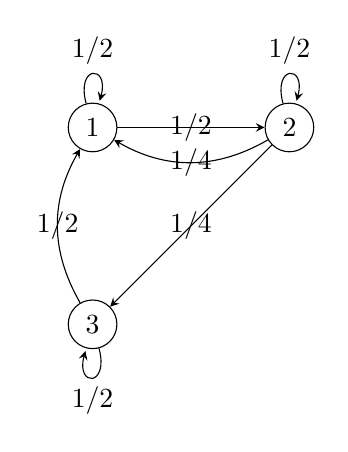
\begin{tikzpicture}[>=stealth, node distance=2.5cm]
\node[circle,draw] (1) {1};
\node[circle,draw,right of=1] (2) {2};
\node[circle,draw,below of=1] (3) {3};

\draw[->] (1) edge[loop above] node{$1/2$} (1)
          (1) edge node{$1/2$} (2);
\draw[->] (2) edge[loop above] node{$1/2$} (2)
          (2) edge[bend left] node{$1/4$} (1)
          (2) edge node{$1/4$} (3);
\draw[->] (3) edge[loop below] node{$1/2$} (3)
          (3) edge[bend left] node{$1/2$} (1);
\end{tikzpicture}
\end{center}

\section*{Perron--Frobenius Theorem}

\begin{theorem*}[T3.8]
Let $A$ be an irreducible nonnegative matrix, and let
\begin{equation}
\rho = \max\{ |\lambda| : \lambda \text{ eigenvalue of } A \}.
\end{equation}
Then:
\begin{enumerate}[label=(\arabic*)]
\item There exist strictly positive left and right eigenvectors $x,y$ such that
\begin{equation}
Ax=\rho x, \qquad y^T A = \rho y^T.
\end{equation}
\item The eigenvalue $\rho$ has algebraic multiplicity one.
\end{enumerate}
\end{theorem*}

Applied to an irreducible stochastic matrix $P$, this implies existence (first part) and uniqueness (second part) of the invariant distribution $\pi$.
\end{document}
\section*{Convergence Ergodicity for Finite Chains}
Note that we could have a matrix with a stationary density $\pi$ where $\mu_n = \mu_0P^n$ does not converge to $\pi$ for all $\mu_0$. For example
\begin{equation}
\end{equation} 


\begin{definition}
A Markov chain is \emph{primitive} if there exists $n$ such that
\begin{equation}
(P^n)_{ij} > 0 \quad \text{for all } i,j.
\end{equation}
\end{definition}

\begin{theorem}[Primitive convergence, T3.1]
Let $P$ generate a primitive Markov chain with invariant distribution $\pi$.
Then for any initial distribution $\mu$,
\begin{equation}
\mu P^n \to \pi
\quad \text{exponentially fast as } n\to\infty.
\end{equation}
\end{theorem}

\begin{proof}[Proof sketch]
Let
\[
d(\mu,\nu)=\frac12\sum_{i=1}^I|\mu_i-\nu_i|
\]
denote total variation distance.

\medskip
\noindent\emph{Step 1.}
For any probability measures $\mu,\nu$,
\[
d(\mu,\nu)\le 1,
\]
with equality attained, for example, when $\mu=e_i$ and $\nu=e_j$, $i\neq j$.

\medskip
\noindent\emph{Step 2.}
Since $P$ is primitive, there exist $m\in\mathbb{N}$ and $\varepsilon>0$ such that
\[
(P^m)_{ij}\ge \varepsilon
\qquad \text{for all } i,j.
\]
Then
\begin{align*}
d(\mu P^m,\nu P^m)
&= \frac12\sum_{j=1}^I
\left|
\sum_{i=1}^I (\mu_i-\nu_i)(P^m)_{ij}
\right| \\
&\le \frac12\sum_{j=1}^I\sum_{i=1}^I
|\mu_i-\nu_i|(P^m)_{ij}.
\end{align*}

Using $\sum_i(\mu_i-\nu_i)=0$ and the uniform lower bound $\varepsilon$, one obtains
\[
d(\mu P^m,\nu P^m)\le (1-\varepsilon)\,d(\mu,\nu).
\]

\medskip
\noindent\emph{Step 3.}
Iterating this contraction,
\[
d(\mu P^{km},\nu P^{km})\le (1-\varepsilon)^k d(\mu,\nu).
\]
Taking $\nu=\pi$ and using invariance $\pi P^m=\pi$ yields exponential convergence.
\end{proof}

Exponential convergence means there exist constants $C<\infty$ and $0<r<1$ such that
\begin{equation}
\|\mu P^n-\pi\|_{\mathrm{TV}}\le C r^n.
\end{equation}

\section*{Ergodic Theorem}

\begin{theorem}[Ergodic theorem, T3.12]
Let $(X_n)$ be an irreducible finite-state Markov chain with invariant distribution $\pi$, and let
$f:\Omega\to\mathbb{R}$ be bounded. Then
\begin{equation}
\frac{1}{n}\sum_{k=0}^{n-1} f(X_k)
\xrightarrow{a.s.}
\sum_{i=1}^I f(i)\,\pi_i.
\end{equation}
\end{theorem}

\end{document}